\section{Conception Devops}
\begin{figure}[h]
   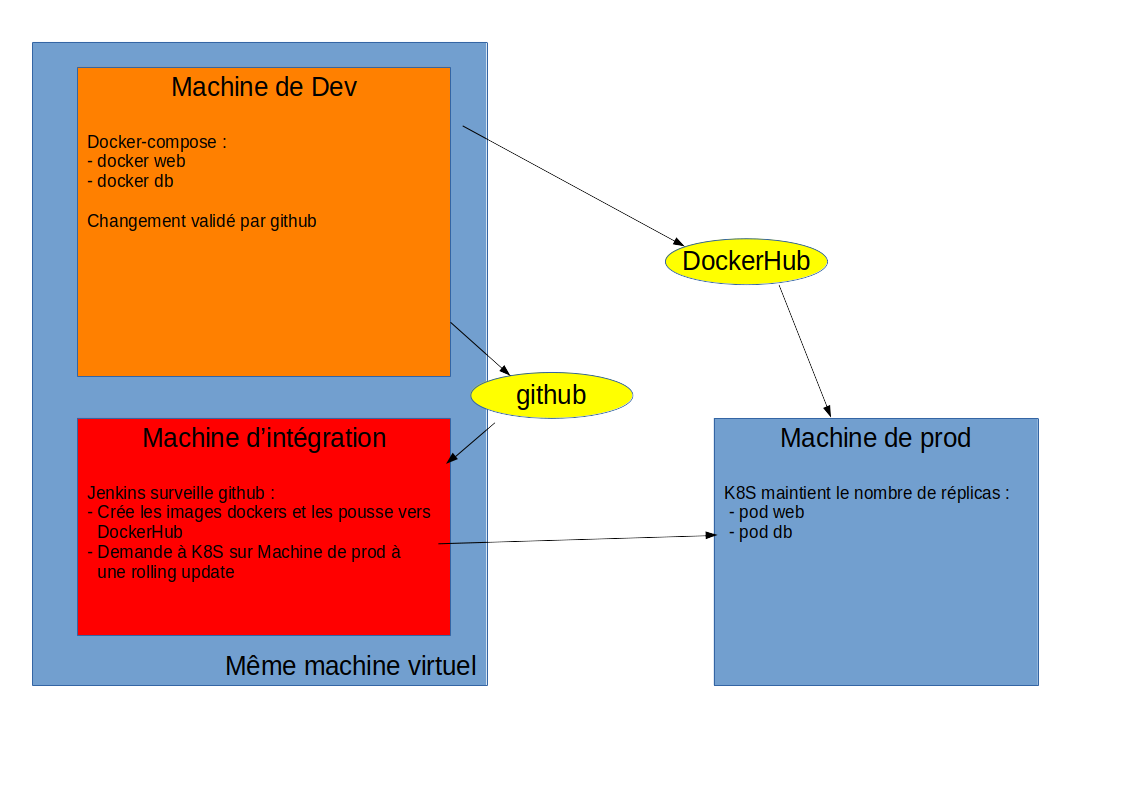
\includegraphics[width=1.0\textwidth]{schema.png}
\end{figure}
\subsection{Gestion de versions}
Tous les fichiers sources et de configuration sont versionné avec git en utilisant github :

\url{https://github.com/RaoulChartreuse/exo_SNCF}


On utilisera 2 branches~ : une branche dev pour l’implémentation des nouvelles fonctionnalités et la branche master pour chaque version validée.

\subsection{Machine de production}
Compte tenue des besoins de disponibilité et de mise à l’échelle (scalling), la conteneurisation retenue est \emph{kubernetes} qui permet justement de gérer le nombre de réplication et de garantir celui-ci.

Compte tenue de l’environnement du projet, nous utiliseront \emph{minikube} et simulerons un ensemble de serveur sur une machine virtuelle de développement.

Liste des pods~:
\begin{itemize}
\item web : un pod de serveurs appache/php
\item db : un pod de serveurs mysql
\end{itemize}

\subsection{Machine de Développement}
Idéalement l’environnement de test doit identique à l’environnement de production. Ici en l’absence de machine de test et avec des ressources limitées à un seul ordinateur, nous utiliseront pour le développement des serveurs dockers obtenue grâce à un \emph{docker compose}.

Liste des serveurs~:
\begin{itemize}
\item web : un docker appache/php
\item db : un docker mysql
\end{itemize}

\subsection{Deploymenent et integration}
La surveillance des dépôts git sera effectuée par un serveur emph{Jenkins}. Dans le cadre des ressources limitées du projet jenkin sera conteneurisé par un conteneur docker sur la machine de développement.

\subsubsection{Mise à jour de la branche dev}
En cas de mise à jour de la branche dev il faut~:
\begin{itemize}
\item Arrêter les conteneurs db
\item Recréer les images des conteneurs à jour grâce à docker compose
\item Lancer les conteneurs à jour
\item Supprimer les images obsolète
\end{itemize}

\subsection{Mise à jour de la branche prod}
Nous utiliserons la fonctionnalité Rolling update de Kubernetes.

\subsection{Création des machines de prod}
Nous automatiserons la création des machines de prod grâce à \emph{Ansible}.
Ici dans le cadre du projet cela ce limitera à la configuration d'une seul machine de prod, l’installation et le déploiement de minikube.

%%% Local Variables:
%%% mode: latex
%%% TeX-master: t
%%% End:

